\section{Ubiquitous Pointing}
%todo:The state of art the eye tracking is changinng discontinously. 
Ubiquitous computing is a concept in software engineering and computer science where computing is made to appear anytime and anywhere. In contrast to desktop computing, ubiquitous computing can occur using any device, in any location, and in any format. A user can interact with the computer, which exists in different forms, laptop, tablets, everyday devices such as a lamp or a TV. The underlying technologies to support ubiquitous computing include Internet, operating system, sensors, microprocessors, \textbf{new  I/O and user interfaces}, networks and so on.  Ubiquitous computing presents challenges in user interface design as contemporary HCI models, whether command-line, menu-driven, or GUI-based, are inappropriate and inadequate to the ubiquitous case. A natural interaction paradigm is important factor for ubiquitous computing emerging. In section \ref{sec:4-PAST}, we present a method to recover the user's pointing gesture, which could be one human-computer interaction model for ubiquitous computing. The use of hand gestures provides an attractive and natural alternative to the traditional cumbersome devices for human computer interaction. 
Recovery of the pointing gestures can help achieve the ease and naturalness desired interaction with general computing device.
%introdcue the scenario with no depth infro and the framework for Ubiquitous pointing

As defined previously in Section \ref{sec:4-PAST}, the fingertip $F$ is collinear with  $T$ and $E$, the pointing direction could be calculated based on the detected fingertip after PAST calibration. To complete the computer-human interaction, there are two solution: (1) a user directly performs a interaction with some input device, which is connected to some computing device, and the input signal is translated to the desired device or (2) a computing device could understand the user's natural behavior and directly translate corresponding signal to the desired device.  In this section, a wearable RGB-D sensor acts as a bridge between the computing device and the human, and the pointing gesture is studied as the potential user interface in a ubiquitous computing scenario.
A wearable sensor can perceive a similar view as the user but it cannot get the same view. To really understand the user's behavior, the sensor has to know exactly where the user is pointing towards. In another words, to calculate where the user is point at in the scene image.
Comparing to eye gaze tracking, the advantage of pointing gesture is: (i) the user could select an area of interesting as potential image for the computing device to understand and (ii) the user could focus on any visual feedback when perform the interaction.  

%the methmatic method to compute the target in the color image
%the main function is: we could estimate where the user is point towards in the color image. 
\subsection{Estimate Target Position}
In the general setup, there is a scene camera to perceive the similar view as the user but it is very clear that the position of the fingertip in the scene camera is not the position of the target. In many ubiquitous computing scenarios, a valid depth map or a tracked known objected does not exist and we could calculate the 3D position of the target and project it to 2D image to calculate the 2D position. As we all know, the eye always rotate and make sure the pupils directly face to the target and the fingertip $F$ is collinear with  $T$ and $E$. So we assume that the 2D position of the fingertip $F$ and that of the target $T$  are at the center of the virtual eye image $I_{e}$, as shown in \figurename{\ref{fig:4-UP:noDepth}}.
\begin{figure}[htb]
	\centering
	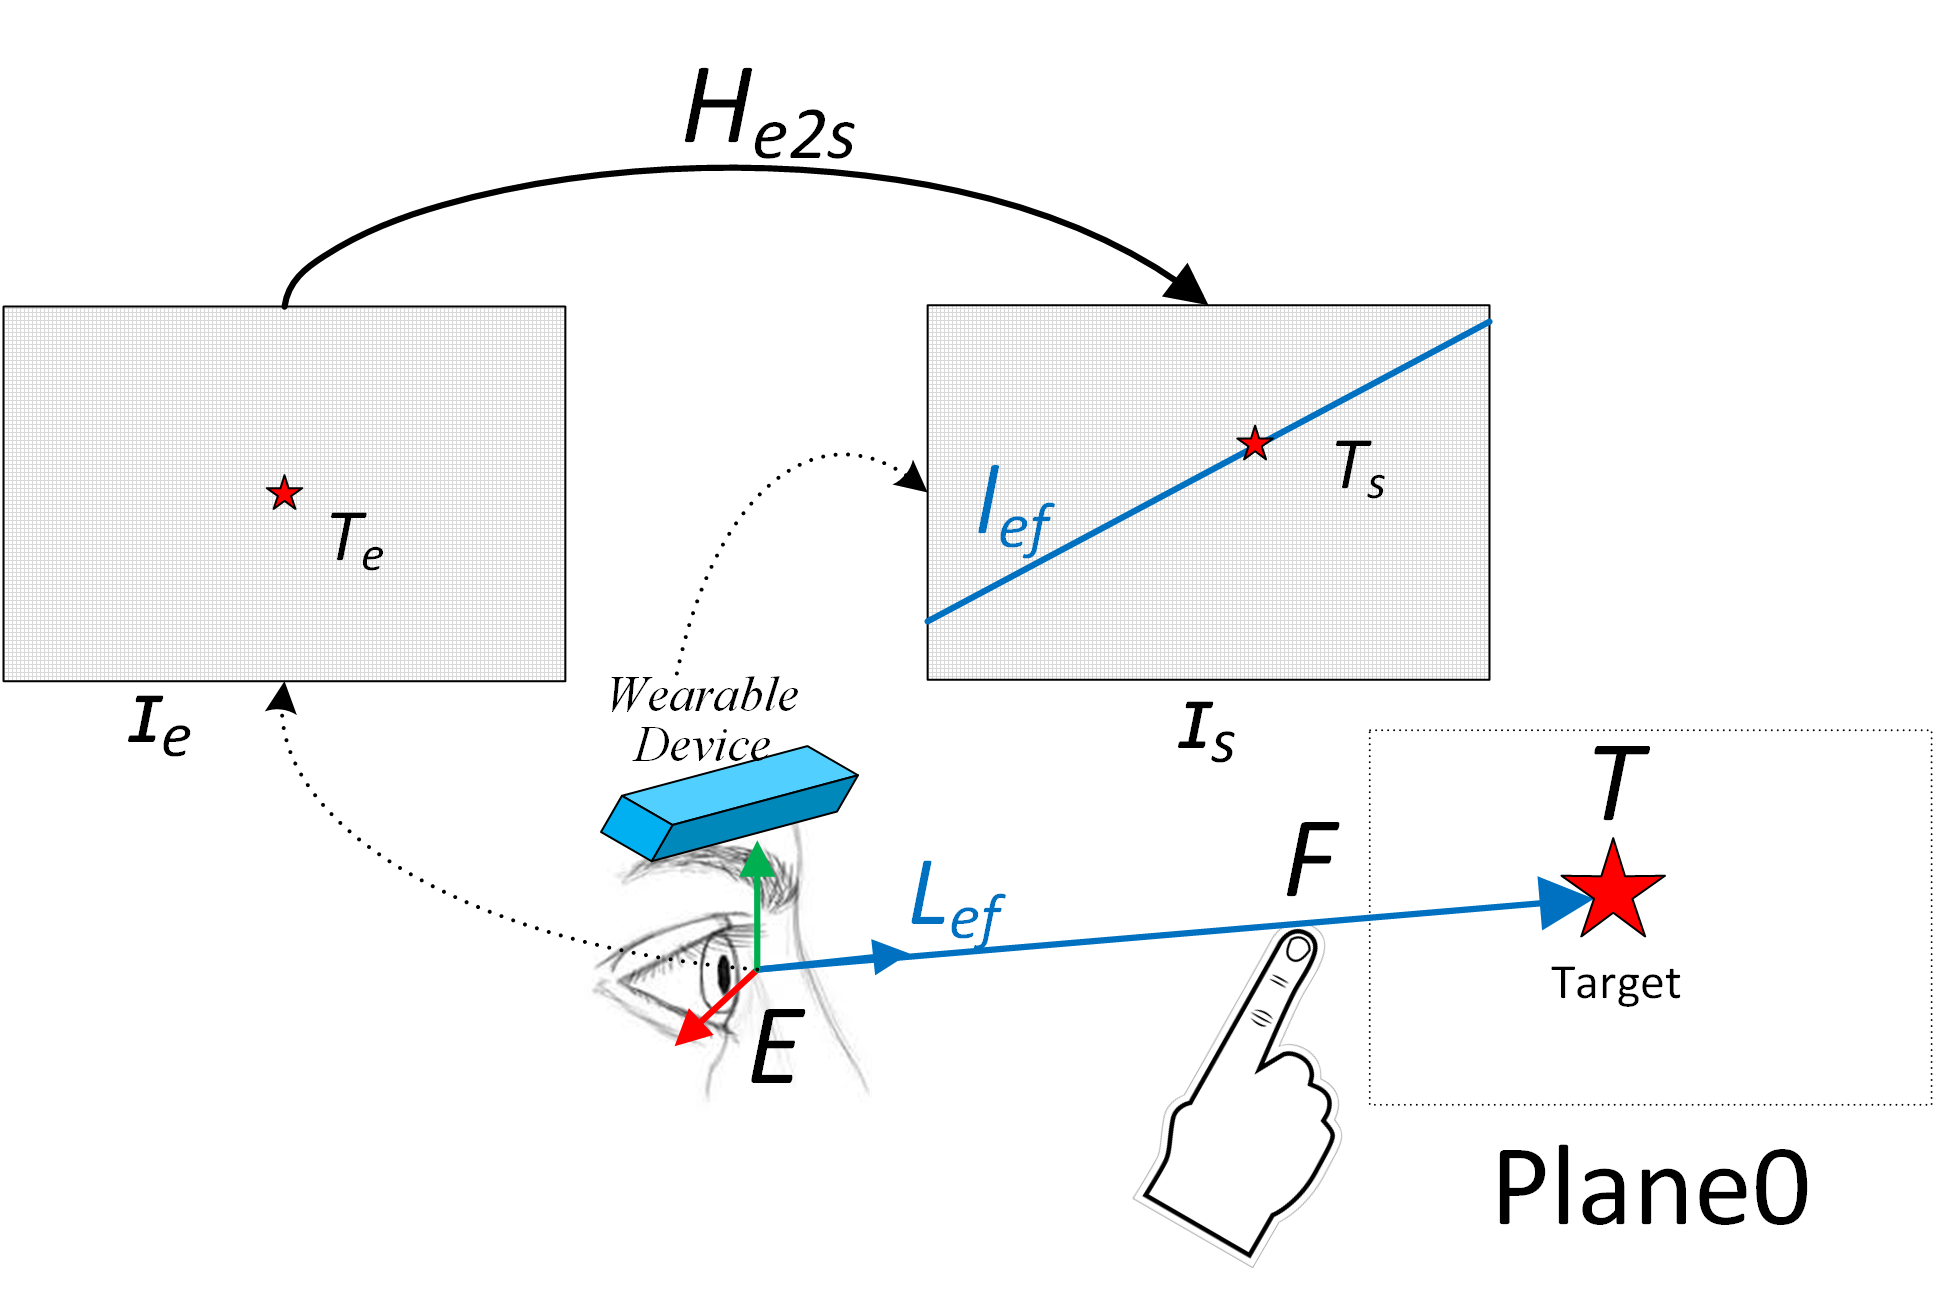
\includegraphics[width = \linewidth]{figures/4-UP/NoDepth.png}
	\caption{The eye camera projects the target $T$  and the finger tip $F$ to the center of the virtual eye image $I_{e}$.  $H_{e2c}$  is the planar homography matrix from the  eye camera to the scene camera on the plane $Plane0$.}
	\label{fig:4-UP:noDepth}
\end{figure}
Based on our assumption, the eye camera looks in the same direction as the line of sight $L_{ef}$. The transformation  $Tran_{d2e}$ of the eye camera relative to the depth camera could be computed based on $E$ and $L_{ef}$ and then we could compute the transformation of the color camera relative to the eye camera. Any target is belong to a plane, and the current $T$ is a part of the plane $Plane0$. 
The planar homography matrix between the eye camera and the scene camera is defined as:
\begin{equation}
\label{eq:homography}
H = R + \frac{1}{d}T{N^T}
\end{equation}
where $R$ and $T$ are the rotation matrix and translation vector of the scene camera relative to the eye camera and $N$ is the normal vector of $Plane0$ and $d$ is a perpendicular distance from $E$ to $Plane0$. As we assumed the whole scene is a large and far-away plane, $d \approx \infty$ and $H=R$.
$T_{s}$ is calculated using:
\begin{equation}
\label{eq:computeTarget}
{T_{s}}= {K_s} \cdot {H_{e2s}} \cdot K_e^{ - 1} \cdot {T_{e}}
\end{equation}
where  $K_s$ and $K_e$ are the scene and eye cameras{\rq} intrinsic parameter matrices. Here, $K_e$ does not influence as the eye camera always projects the target ,which the user is focusing on, to the center  of the virtual eye image $I_{e}$. So the parameters of the eye camera are set as the scene camera. $l_{ef}$ is the projection of $L_{ef}$ in the scene image and the target result could be optimized by the closest point along $l_{ef}$ to the current $T_s$. Then the computing device knows where the user is pointing in the scene camera.

%Analysis of the method
\subsection{Evaluation of the method}
1. The user could point to the target and looking at a different direction to read the information shown on the HMD  2. The user could draw a shape overlop the color image to select the area of interesting
In this scenario, we perform the simulation at three different configurations:(i) $P_{eye}$ = [0.16112,  -5.19904,  -2.04530] (cm) and $d_{finger}$ = 20cm; (ii) $P_{eye}$ = [0.16112,  -5.19904,  -2.04530] (cm) and $d_{finger}$ = 30cm; (iii) $P_{eye}$ = [0.16212 , -3.19894 , -2.04380] (cm) and $d_{finger}$ = 30cm;
We calculate the 2D position of the finger $p_{finger}$ and target $p_{target}$ in the color image and $Target_{color}$  is computed using the proposed method. The Raw offset is the offset between $p_{finger}$ and $p_{target}$ while the offset of OurMethod is the offset between $Target_{color}$ and $p_{target}$. Under each configuration, we increase $d_{target}$ from 1 meter to 10 meter by a 0.5m step size and compute the average offset of the 2400 targets in every step. The results are shown in Figure \ref{fig:4-UP:simulateResi},\ref{fig:4-UP:simulateResii} and \ref{fig:4-UP:simulateResiii}.  
From the simulation result, it is very obvious the offsets of OurMethod are much smaller than the Raw offset. As $d_{target}$ increases, the offset of OurMethod decreases and the Raw increase. From Figure \ref{fig:4-UP:simulateResi}, the offset decreases 78\%, from 360 to 81, in the worst case and 94\% on average from 419 to 22, under configuration i.  Under configuration ii, it 
is 60\%, from 202 to 81, in the worst case and 92\% on average from 261 to 22. The offset decreases from 143 to 57, about 60\%, in the worst case, and from 185 to 15, 92\% on average under configuration iii.
The worst case always happens at 1m, but the error makes sense as we assumed the whole scene as a large and far-away plane.\\
Based on image resolution and field of view of the color camera, we could compute the pixel spacing in centimeters at different distances. If we convert the raw offset into real world distance, the offsets increase greatly, from 38 cm to 412 cm under configuration i, from 24 cm to 277 cm under configuration ii and from 15 cm to 206 cm under configuration iii. 
However, the offset of our method is very stable after converting to real world distance. 
The real distance offset in the three configurations are about 8.4cm, 8.cm and 6cm, respectively. Hence, our method can estimate the position of the target the user is pointing to very accurately, and has potential to be used as a natural user interface for ambient devices.
The offset between configuration i and configuration ii, is similar, so where the user put their hand does not affect the accuracy of our method. The offset under configuration iii decreased compared to the others. It is because the distance from $P_{eye}$ to RGB-D sensor declined from 5.6 cm to 3.8 cm. To rectify this, we can try to affix the RGB-D sensor closer to the center of the user eyes for more accurate results. 
\begin{figure} [h]
	\centering
	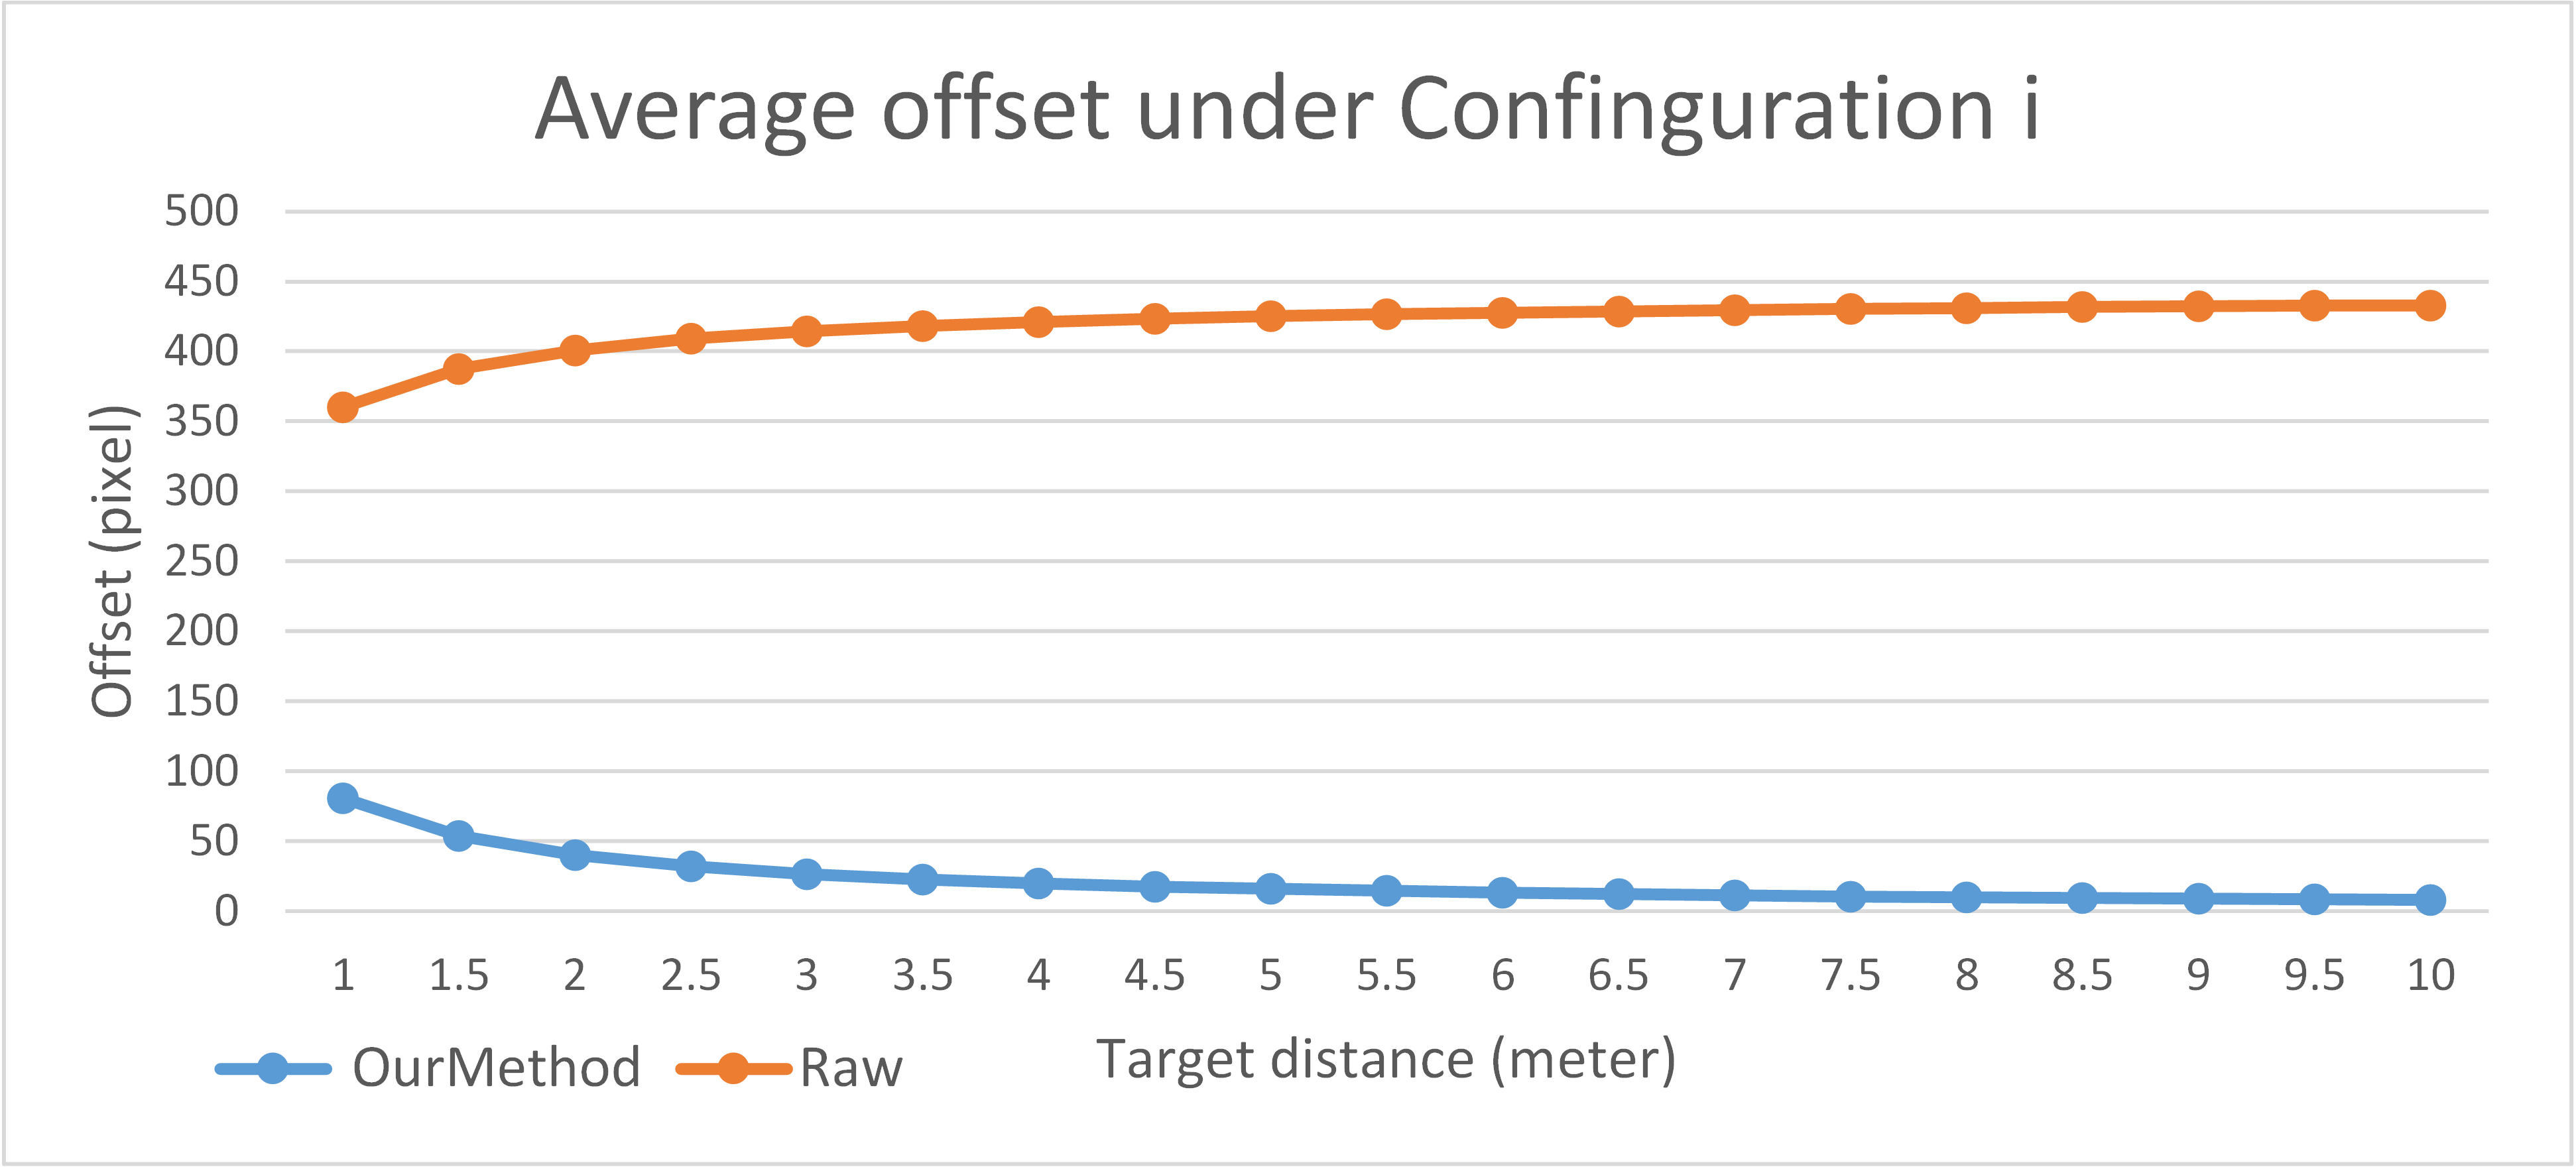
\includegraphics[width= \linewidth]{figures/4-UP/simulationResi.png}
	\caption{The average offset of OurMethod and the Raw in different distance under configuration i.}
	\label{fig:4-UP:simulateResi}
\end{figure}
\begin{figure} [h]
	\centering
	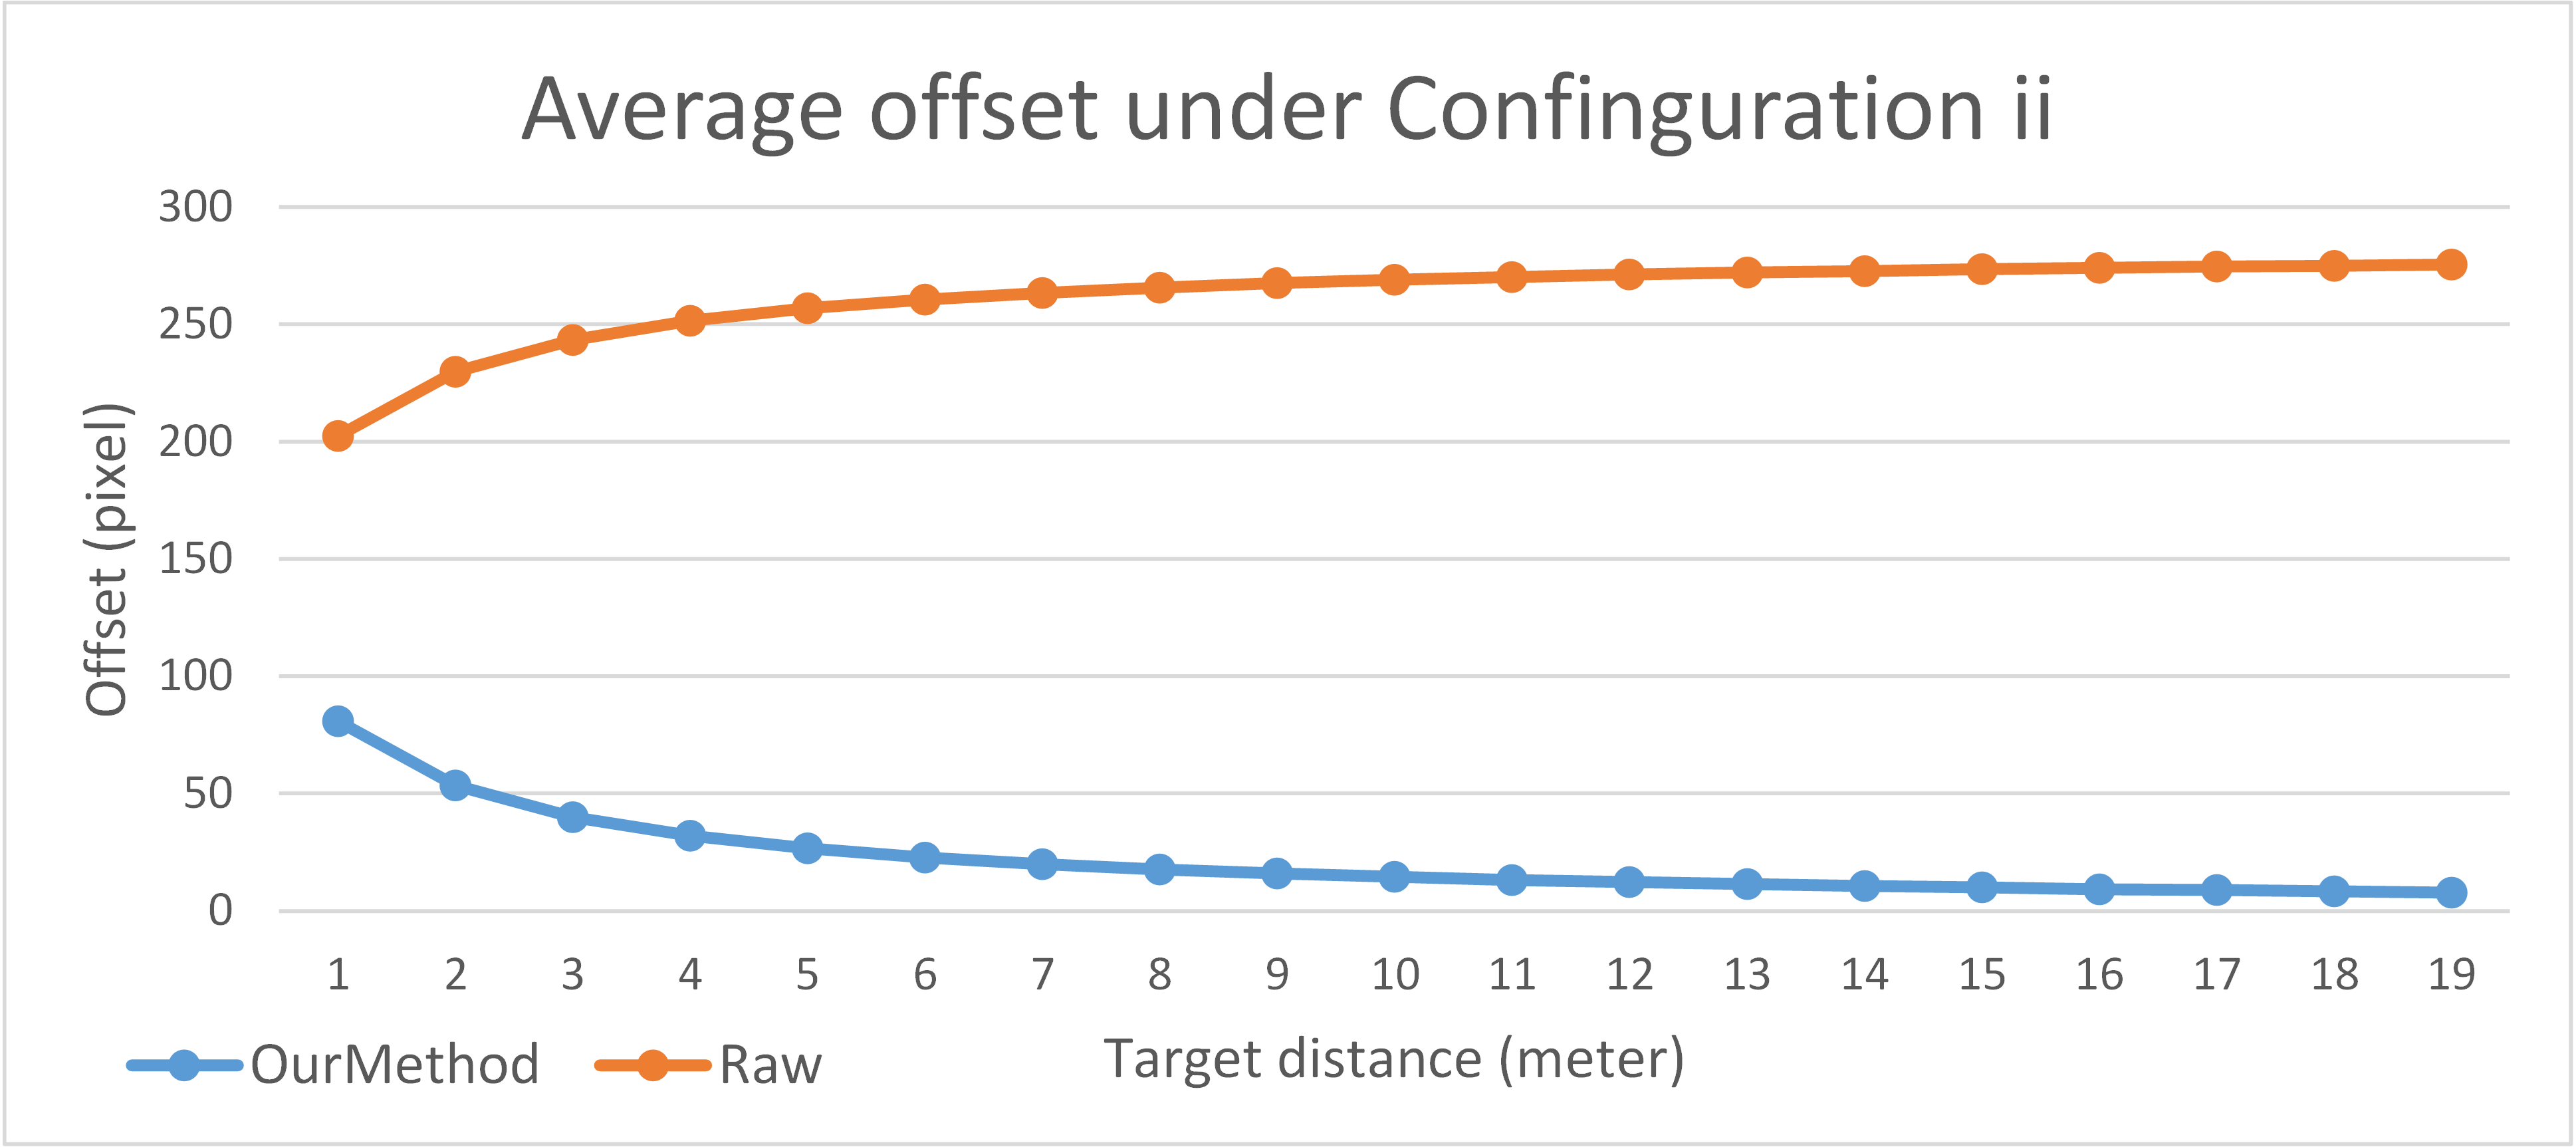
\includegraphics[width= \linewidth]{figures/4-UP/simulationResii.png}
	\caption{The average offset of OurMethod and the Raw in different distance under configuration ii.}
	\label{fig:4-UP:simulateResii}
\end{figure}
\begin{figure} [h]
	\centering
	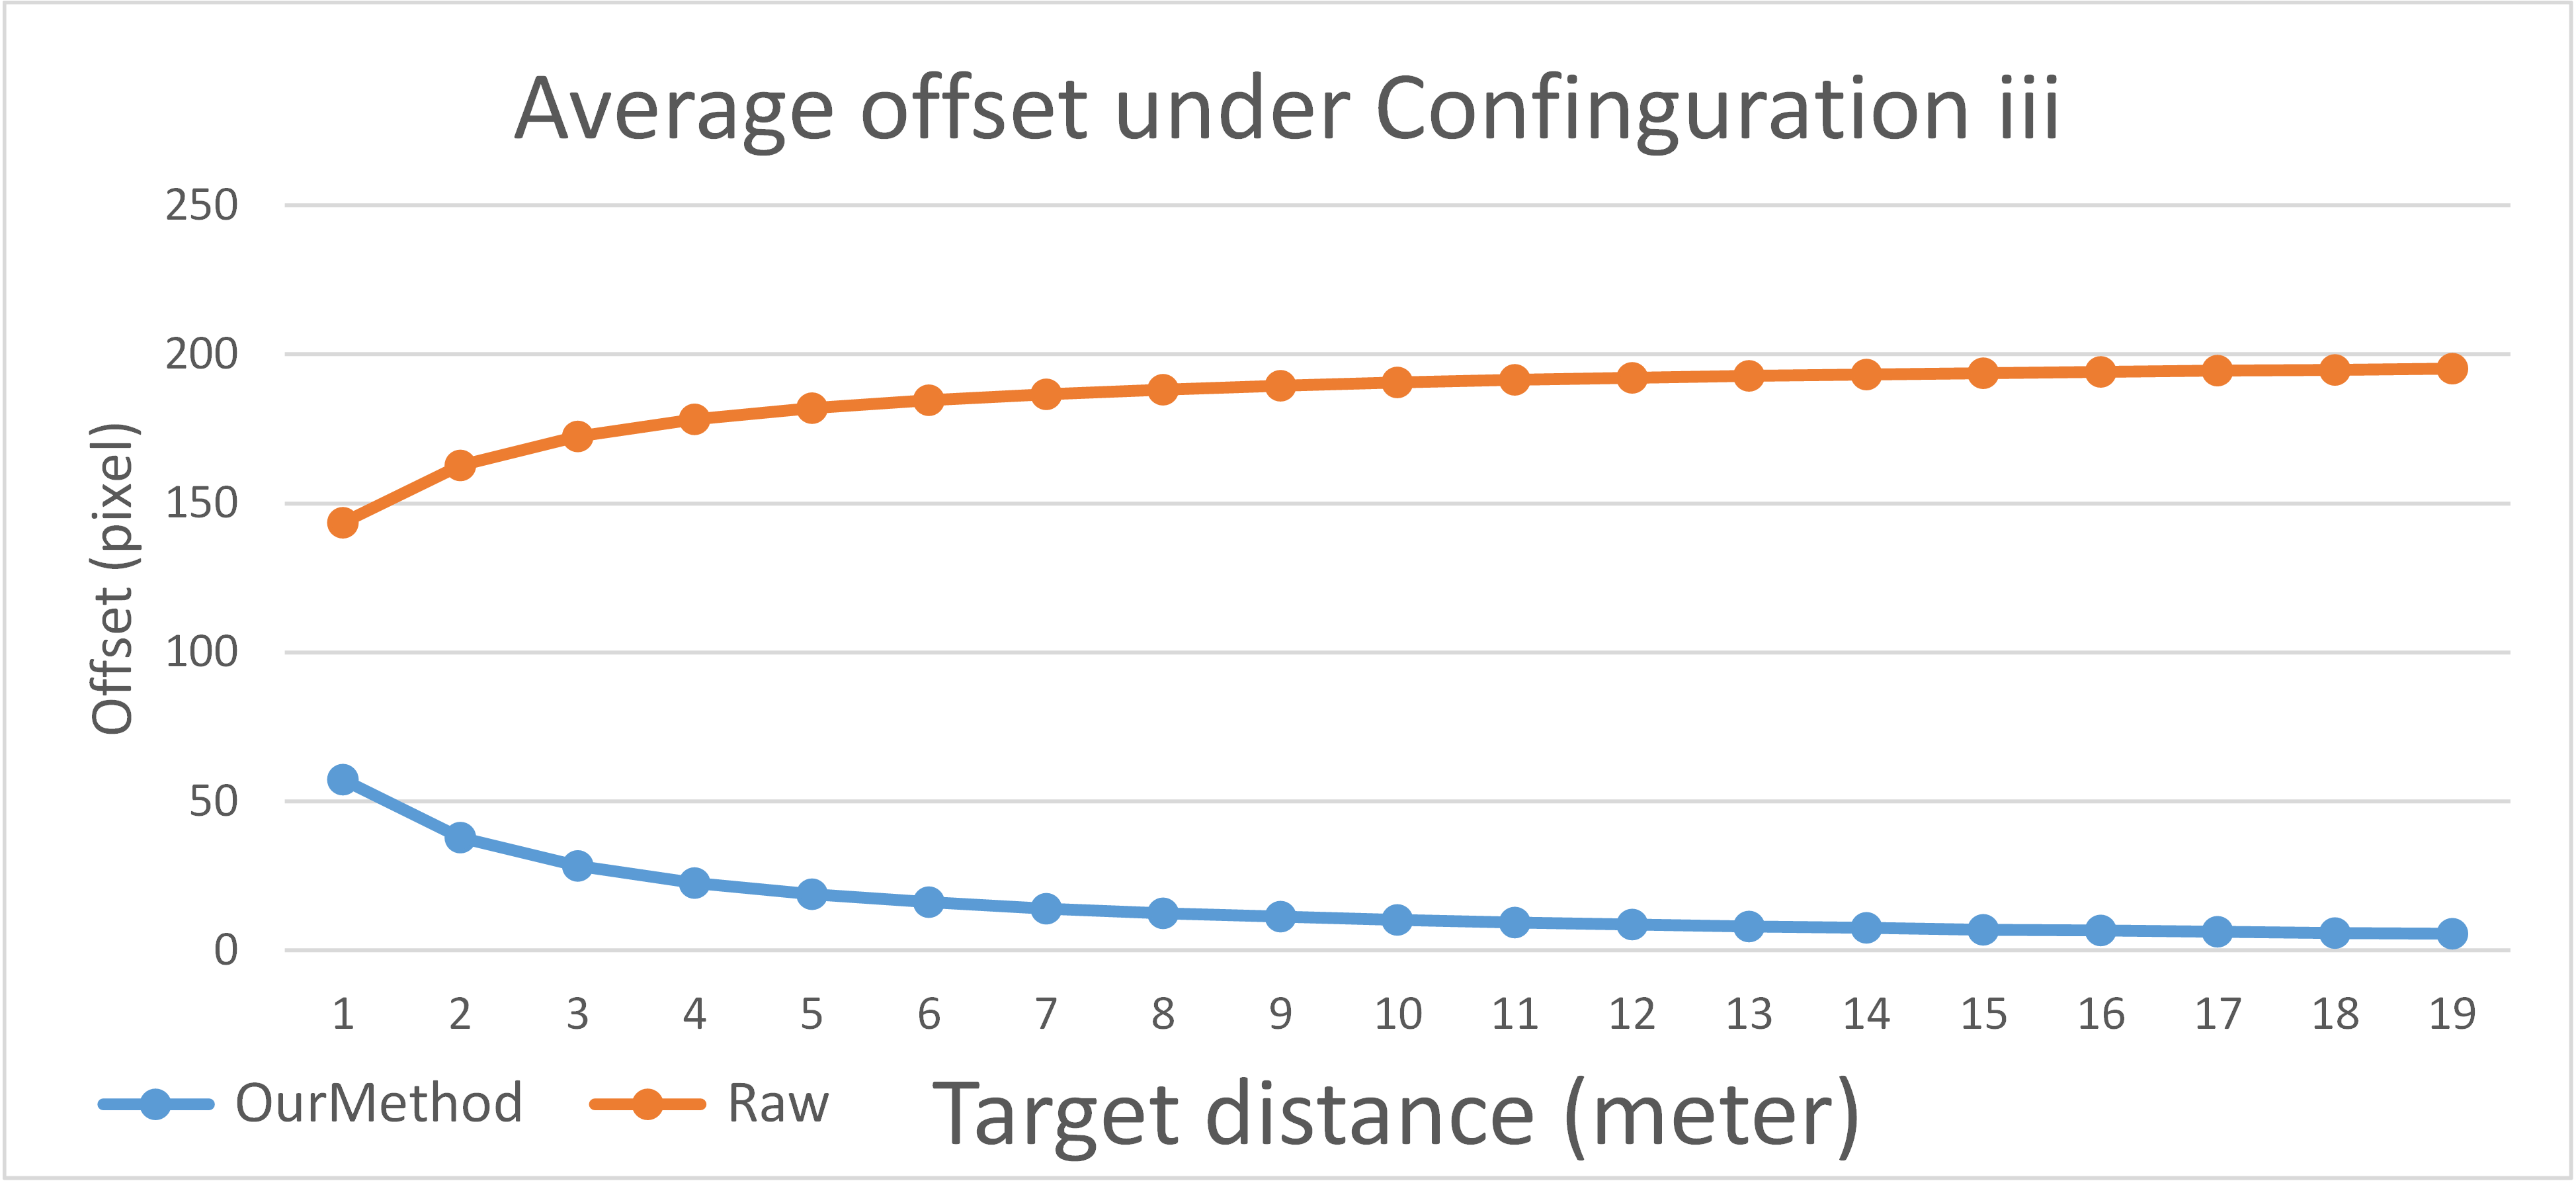
\includegraphics[width= \linewidth]{figures/4-UP/simulationResiii.png}
	\caption{The average offset of OurMethod and the Raw in different distance under configuration iii.}
	\label{fig:4-UP:simulateResiii}
\end{figure}
%potential application with this method
\subsection{Potential Application}

The computer could try to search based on the whole scene image, it is not doable  as there are two many information. The search need a good initial value for the research.
